% ============================================================================
%  Trabalho de Calculo Numerico - Pseudoinversa de Moore-Penrose
%  IFCE - Engenharia de Computacao e Telecomunicacoes
%  Autores: Vinicius Menezes Monte e Marcelo Flávio de Carvalho Frota Porto  |  Prof. Dr. Francisco Aquino  |  Fortaleza, 2026
%  Formatacao ABNT: Times 12pt, espacamento 1,5, margens 3-2-3-2 cm
%  Compilar: pdflatex (3x para sumario)
% ============================================================================
\documentclass[12pt,a4paper,oneside]{report}

\usepackage[utf8]{inputenc}
\usepackage[T1]{fontenc}
% babel-pt indisponivel neste ambiente: nomes em portugues definidos manualmente
\renewcommand{\figurename}{Figura}
\renewcommand{\tablename}{Tabela}
\usepackage{mathptmx}            % fonte Times New Roman (texto e matematica)
\usepackage{microtype}
% sem padroes de hifenizacao PT: desliga hifenizacao e ajusta espacamento
\hyphenpenalty=10000 \exhyphenpenalty=10000
\tolerance=2500 \emergencystretch=3em \hbadness=10000
\usepackage[a4paper,top=3cm,bottom=2cm,left=3cm,right=2cm]{geometry}
\usepackage{setspace}
\usepackage{amsmath,amssymb}
\usepackage{mathtools}
\usepackage{graphicx}
\usepackage{booktabs}
\usepackage{listings}
\usepackage{xcolor}
\usepackage{fancyhdr}
\usepackage{indentfirst}
\usepackage[hidelinks]{hyperref}
\usepackage{caption}

% ---- espacamento e paragrafo ABNT ----
\onehalfspacing
\setlength{\parindent}{1.25cm}
\setlength{\parskip}{0.2em}

% ---- numeracao de paginas no canto superior direito ----
\pagestyle{fancy}
\fancyhf{}
\fancyhead[R]{\thepage}
\renewcommand{\headrulewidth}{0pt}
\setlength{\headheight}{15pt}
\fancypagestyle{plain}{%
  \fancyhf{}\fancyhead[R]{\thepage}\renewcommand{\headrulewidth}{0pt}}

% ---- titulos de capitulo/secao mais sobrios ----
\usepackage{titlesec}
\titleformat{\chapter}[hang]{\normalfont\large\bfseries}{\thechapter}{12pt}{\large}
\titlespacing*{\chapter}{0pt}{-10pt}{14pt}
\titleformat{\section}{\normalfont\bfseries}{\thesection}{8pt}{}
\titleformat{\subsection}{\normalfont\bfseries\itshape}{\thesubsection}{8pt}{}

% ---- macros ----
\newcommand{\norm}[1]{\left\lVert #1 \right\rVert}
\newcommand{\T}{^{\mathsf{T}}}
\newcommand{\Ap}{A^{+}}
\newcommand{\R}{\mathbb{R}}

% ---- estilo de codigo ----
\definecolor{codegray}{rgb}{0.5,0.5,0.5}
\definecolor{codeblue}{rgb}{0.10,0.20,0.55}
\definecolor{codebg}{rgb}{0.97,0.97,0.97}
\lstset{
  basicstyle=\ttfamily\footnotesize,
  keywordstyle=\color{codeblue}\bfseries,
  commentstyle=\color{codegray}\itshape,
  backgroundcolor=\color{codebg},
  frame=single, rulecolor=\color{codegray},
  numbers=left, numberstyle=\tiny\color{codegray},
  breaklines=true, showstringspaces=false,
  language=Python, tabsize=2, xleftmargin=14pt
}

\begin{document}
\pagestyle{empty}
\pagenumbering{Alph}

% ============================ CAPA ==========================================
\thispagestyle{empty}
\begin{center}
  {\large\bfseries INSTITUTO FEDERAL DE EDUCAÇÃO, CIÊNCIA E TECNOLOGIA DO CEARÁ -- IFCE}\\[2pt]
  {\normalsize Cursos de Engenharia de Computação e de Telecomunicações}\\[2pt]
  {\normalsize Disciplina: Cálculo Numérico}

  \vspace{4.0cm}

  {\normalsize VINÍCIUS MENEZES MONTE}\\[2pt]
  {\normalsize MARCELO FLÁVIO DE CARVALHO FROTA PORTO}

  \vspace{3.5cm}

  {\large\bfseries CÁLCULO NUMÉRICO E CIÊNCIA DA COMPUTAÇÃO:}\\[4pt]
  {\large\bfseries história e fundamentos da Pseudoinversa de Moore-Penrose}

  \vfill

  {\normalsize Fortaleza -- Ceará\\ 2026}
\end{center}
\clearpage

% ====================== FOLHA DE ROSTO ======================================
\pagenumbering{arabic}
\thispagestyle{empty}
\begin{center}
  {\normalsize VINÍCIUS MENEZES MONTE}\\[2pt]
  {\normalsize MARCELO FLÁVIO DE CARVALHO FROTA PORTO}

  \vspace{4.5cm}

  {\large\bfseries CÁLCULO NUMÉRICO E CIÊNCIA DA COMPUTAÇÃO:}\\[4pt]
  {\large\bfseries história e fundamentos da Pseudoinversa de Moore-Penrose}
\end{center}

\vspace{2.0cm}

\hfill\begin{minipage}{0.55\textwidth}
\singlespacing\small
Trabalho apresentado à disciplina de Cálculo Numérico dos cursos de Engenharia de
Computação e de Telecomunicações do Instituto Federal do Ceará (IFCE), como requisito
parcial de avaliação.

\vspace{0.8cm}
Orientador: Prof.\ Dr.\ Francisco Aquino.
\end{minipage}

\vfill
\begin{center}{\normalsize Fortaleza -- Ceará\\ 2026}\end{center}
\clearpage

% ========================== SUMARIO =========================================
\thispagestyle{empty}
{\singlespacing
\renewcommand{\contentsname}{\centerline{\normalfont\large\bfseries SUMÁRIO}}
\tableofcontents}
\thispagestyle{empty}
\clearpage

% ========================= INTRODUCAO =======================================
\pagestyle{fancy}
\chapter*{Introdução}
\addcontentsline{toc}{chapter}{Introdução}

O cálculo numérico pode ser definido como o conjunto de métodos e algoritmos que permitem
resolver, de forma aproximada e por meio de máquinas digitais, problemas matemáticos que
raramente possuem solução analítica fechada (BURDEN; FAIRES, 2015; CHAPRA; CANALE, 2016). Como observa Aquino (2020), trata-se de uma
disciplina de cunho eminentemente prático, voltada a engenheiros e cientistas que usam os
métodos numéricos como ferramenta para a resolução de problemas reais. Equações não
lineares, sistemas lineares de grande porte, integração de funções sem primitiva conhecida e
ajuste de modelos a dados experimentais são situações cotidianas em que a resposta exata é
inacessível e a aproximação controlada torna-se indispensável.

Para a Engenharia de Computação e de Telecomunicações, esse ferramental faz parte do dia a dia. Simulação de circuitos, processamento de sinais, codificação de canal, otimização de redes e aprendizado de máquina apoiam-se fortemente em operações numéricas sobre matrizes e vetores. Há aí também uma relação histórica: o cálculo numérico amadureceu junto com a ciência da computação. A necessidade de resolver problemas grandes foi um dos motores da construção das primeiras máquinas digitais, e essas máquinas tornaram viáveis métodos antes impraticáveis em escala manual (VON NEUMANN; GOLDSTINE, 1947; CERUZZI, 2003).

\noindent\textbf{Objetivo geral.} Analisar a história do cálculo numérico e sua relação com a
ciência da computação, aprofundando um tópico específico da disciplina: a \emph{pseudoinversa
de Moore-Penrose}.

\noindent\textbf{Objetivos específicos.} (i) descrever marcos históricos relevantes do cálculo
numérico; (ii) relacionar o desenvolvimento de métodos numéricos com a evolução de algoritmos
e hardware; (iii) estudar em profundidade a pseudoinversa, sua fundamentação, algoritmo e
implementação; e (iv) discutir suas aplicações em Engenharia de Computação e Telecomunicações.

A pseudoinversa foi escolhida por um motivo concreto. Ela estende a ideia de inversa para os casos em que a inversa clássica não existe (matrizes retangulares ou singulares) e fornece, em termos precisos, a solução de mínimos quadrados de menor norma para sistemas lineares gerais (PENROSE, 1955; GOLUB; VAN LOAN, 2013). É um tema que liga a Álgebra Linear ao cálculo numérico e que aparece com frequência no ajuste de curvas, na compressão por decomposição em valores singulares (SVD) e em problemas de estimação.

O Capítulo~1 traça um panorama histórico do cálculo numérico e de sua ligação com a computação. O Capítulo~2 trata da pseudoinversa em detalhe: contexto histórico, fundamentação teórica, o algoritmo baseado na SVD, a implementação, os resultados e as aplicações em engenharia. O Capítulo~3 reflete sobre a relação entre cálculo numérico, computação e engenharia, e a Conclusão retoma os objetivos do trabalho.

% ===================== CAPITULO 1 - HISTORIA ================================
\chapter{História do cálculo numérico e sua relação com a computação}

Este capítulo traça um panorama histórico do cálculo numérico, com atenção à evolução dos métodos e à sua ligação com a ciência da computação. Há um padrão que se repete: muitos métodos numéricos nasceram de necessidades práticas de cálculo e logo esbarraram no limite do que uma pessoa consegue computar à mão. Esse limite foi sendo deslocado por tabelas, instrumentos mecânicos, computadores humanos e, finalmente, máquinas digitais.

\section{Marcos históricos: da Antiguidade ao século XIX}

A ideia de aproximar grandezas que não se conseguia calcular exatamente é antiga. No século
III a.C., Arquimedes estimou o valor de $\pi$ por polígonos inscritos e circunscritos,
estreitando o intervalo entre os perímetros à medida que aumentava o número de lados -- um
procedimento de refinamento sucessivo que é, em essência, um método numérico (BOYER;
MERZBACH, 2011). Civilizações babilônica, chinesa, indiana e árabe desenvolveram algoritmos
para extrair raízes e resolver equações; a latinização do nome de al-Khwarizmi, ligada a seu
tratado aritmético do século IX, está na origem do termo \emph{algoritmo}. Métodos que ainda hoje estudamos têm raízes igualmente antigas: procedimentos equivalentes à eliminação para sistemas lineares aparecem no tratado chinês \emph{Nove Capítulos sobre a Arte Matemática}, e métodos babilônicos de extração de raízes antecipam ideias que hoje reconhecemos em iterações do tipo Newton-Heron (BOYER; MERZBACH, 2011).

Entre os séculos XVII e XIX, o desenvolvimento do cálculo diferencial e integral por Newton e
Leibniz forneceu a base teórica sobre a qual floresceram os métodos numéricos modernos.
Surgiram técnicas que ainda hoje integram qualquer curso da disciplina: o método de
Newton-Raphson para raízes de equações, as fórmulas de interpolação de Newton e de Lagrange,
a quadratura para integração e o método dos mínimos quadrados. Nesse último caso, a atribuição
histórica exige cuidado: Legendre publicou a formulação em 1805, enquanto Gauss afirmou tê-la
usado antes e a desenvolveu em trabalhos de astronomia e geodesia publicados a partir de 1809
(STIGLER, 1986). É justamente dessa tradição dos mínimos quadrados que, mais tarde, emergiria
a pseudoinversa. Nesse período, a ``computação'' era manual e apoiava-se em extensas tabelas de
logaritmos e funções trigonométricas, laboriosamente calculadas e publicadas. Foi também nesse
espírito que Charles Babbage anunciou, em 1822, a \emph{Máquina Diferencial}, projetada para
automatizar tabulações por diferenças finitas; a automação eletrônica de uso geral, porém, só se
difundiria no século XX (BABBAGE, 1822; CERUZZI, 2003).

Muitos dos métodos que estruturam a disciplina de Cálculo Numérico amadureceram ao longo desse percurso. A eliminação gaussiana e suas variantes (as decomposições LU e de Cholesky) sistematizaram a resolução de sistemas lineares; métodos iterativos como os de Jacobi e de Gauss-Seidel deram alternativas para sistemas grandes; e técnicas de autovalores, como o método da potência e o algoritmo QR, passaram a integrar a base da álgebra linear numérica moderna (GOLUB; VAN LOAN, 2013).

\section{O século XX e o surgimento dos computadores digitais}

Na primeira metade do século XX, antes dos computadores eletrônicos, cálculos de grande porte
para balística, meteorologia e física nuclear eram realizados por equipes de \emph{computadores
humanos} -- pessoas que executavam contas com lápis, tabelas e calculadoras mecânicas e
eletromecânicas. A Segunda Guerra Mundial acelerou enormemente essa demanda, tornando
evidente a necessidade de automatizar o cálculo.

Um exemplo do novo patamar de cálculo que as máquinas tornaram possível é o método de Monte Carlo. A técnica foi consolidada em Los Alamos no pós-guerra, em problemas de física matemática e transporte de partículas, e descrita classicamente por Metropolis e Ulam (1949). É uma técnica que ganha utilidade prática com bastante poder de cálculo, e Aquino (2020) a apresenta no capítulo final de seu livro como exemplo de como a simulação numérica ampliou o alcance da engenharia.

A resposta veio por vários caminhos, sem uma única linha de sucessão: o ABC foi uma máquina eletrônica digital de propósito específico, o Colossus foi decisivo para criptoanálise, e o ENIAC, apresentado publicamente em 1946, tornou-se marco da computação eletrônica de propósito geral (CERUZZI, 2003). Em paralelo, o modelo teórico da máquina universal de Turing deu uma formulação abstrata para o conceito de computação (TURING, 1937). Desde o início, três coisas andaram juntas: a necessidade de resolver numericamente equações diferenciais e sistemas lineares grandes, o desenvolvimento de algoritmos eficientes e o crescimento da computação como área própria. Em 1947, von Neumann e Goldstine publicaram um dos primeiros estudos sistemáticos sobre erros de arredondamento na resolução de sistemas lineares, o que ajudou a firmar a \emph{análise numérica} como campo de pesquisa; mais tarde, James Wilkinson aprofundaria a análise de estabilidade (VON NEUMANN; GOLDSTINE, 1947; WILKINSON, 1963).

\section{A era dos computadores pessoais e o cálculo numérico atual}

A popularização dos computadores pessoais e das estações de trabalho, a partir das décadas de
1970 e 1980, levou o cálculo numérico para fora dos grandes centros de pesquisa. Linguagens e
ambientes voltados à computação científica se multiplicaram: Fortran, C, C++, Pascal e,
depois, ambientes interativos como o MATLAB, criado por Cleve Moler como uma interface para
rotinas de álgebra linear então disponíveis em LINPACK e EISPACK, além de Scilab e Python com
as bibliotecas NumPy e SciPy (MOLER, s.d.). Por trás desses ambientes, bibliotecas numéricas
como BLAS e LAPACK passaram a fornecer uma base comum para grande parte do software de álgebra
linear científica (ANDERSON et al., 1999).

Nem todo avanço veio do hardware; alguns dos mais importantes foram algorítmicos. O caso mais conhecido é a Transformada Rápida de Fourier (FFT), popularizada por Cooley e Tukey em 1965, que reduziu o custo da transformada discreta de Fourier de $O(n^2)$ para $O(n\log n)$ em casos estruturados. Esse algoritmo foi decisivo para o processamento digital de sinais e para aplicações em telecomunicações e compressão (COOLEY; TUKEY, 1965). Também em 1965, Golub e Kahan publicaram um algoritmo estável para calcular valores singulares e pseudoinversas (GOLUB; KAHAN, 1965).

O livro-texto desta disciplina (AQUINO, 2020) é um bom exemplo dessa cultura: usa o Scilab como ferramenta e prefere uma abordagem prática, apresentando cada método junto aos recursos que o tornam aplicável. O que importa reter é que o avanço da computação permitiu usar em larga escala métodos antes impraticáveis à mão. A pseudoinversa ilustra bem isso: sua formulação algébrica é de 1920, mas seu uso computacional amplo foi favorecido pelos algoritmos estáveis de SVD de Golub e Kahan (1965) e de Golub e Reinsch (1970). É esse o tema do próximo capítulo.

% ===================== CAPITULO 2 - PSEUDOINVERSA ===========================
\chapter{Pseudoinversa de Moore-Penrose}

\section{Contexto histórico}

A pseudoinversa, ou inversa generalizada, responde a uma pergunta natural: se a inversa
clássica $A^{-1}$ só existe para matrizes quadradas e não singulares, o que fazer quando $A$
é retangular ou singular? A primeira formulação algébrica explícita, na literatura de matrizes,
é atribuída a Eliakim Hastings Moore, que em 1920 apresentou à \emph{American Mathematical
Society} a noção de ``recíproca geral'' de uma matriz qualquer (MOORE, 1920; BEN-ISRAEL;
GREVILLE, 2003). O trabalho de Moore, contudo, empregava notação pouco difundida e permaneceu
relativamente obscuro por décadas.

O conceito foi redescoberto de forma independente em problemas aplicados, notadamente por Bjerhammar em geodésia no início da década de 1950, e depois por Roger Penrose, em 1955 (BJERHAMMAR, 1951; PENROSE, 1955). Penrose mostrou que, para toda matriz $A$, existe uma \emph{única} matriz $\Ap$ que satisfaz quatro equações simples, hoje chamadas de condições de Moore-Penrose. Essa caracterização reuniu as abordagens anteriores e fixou o nome ``pseudoinversa de Moore-Penrose''. Faltava ligar a teoria à prática computacional, e a decomposição em valores singulares foi decisiva para isso: os algoritmos de Golub e Kahan (1965) e de Golub e Reinsch (1970) tornaram o cálculo de valores singulares e soluções de mínimos quadrados numericamente estável, base para implementações modernas de $\Ap$ (GOLUB; KAHAN, 1965; GOLUB; REINSCH, 1970; GOLUB; VAN LOAN, 2013).

\section{Fundamentação teórica}

\subsection{Definição e as quatro condições de Moore-Penrose}

Dada uma matriz $A \in \R^{m\times n}$, a pseudoinversa $\Ap \in \R^{n\times m}$ é a única
matriz que satisfaz as quatro condições:
\begin{equation}
\text{(1) } A\Ap A = A; \quad
\text{(2) } \Ap A \Ap = \Ap; \quad
\text{(3) } (A\Ap)\T = A\Ap; \quad
\text{(4) } (\Ap A)\T = \Ap A.
\label{eq:mp}
\end{equation}
As duas primeiras generalizam a relação $A A^{-1} A = A$ da inversa clássica; as duas últimas
exigem que os produtos $A\Ap$ e $\Ap A$ sejam matrizes simétricas. Em conjunto, essas condições
fazem de $A\Ap$ e $\Ap A$ projeções ortogonais, respectivamente, sobre o espaço coluna de $A$ e
sobre o espaço linha de $A$ (STRANG, 2006; GOLUB; VAN LOAN, 2013). Quando $A$ é quadrada e invertível, verifica-se que $\Ap = A^{-1}$, de modo que a
pseudoinversa é, de fato, uma extensão do conceito de inversa.

\subsection{Cálculo pela decomposição em valores singulares}

A forma numericamente robusta de obter $\Ap$ parte da decomposição em valores singulares
(SVD). Toda matriz $A \in \R^{m\times n}$ admite a fatoração
\begin{equation}
A = U\,\Sigma\,V\T,
\label{eq:svd}
\end{equation}
em que $U \in \R^{m\times m}$ e $V \in \R^{n\times n}$ são ortogonais e
$\Sigma \in \R^{m\times n}$ é ``diagonal'', com entradas
$\sigma_1 \ge \sigma_2 \ge \dots \ge \sigma_r > 0$ (os valores singulares) e zeros nas
demais posições, onde $r = \operatorname{posto}(A)$. A pseudoinversa é então
\begin{equation}
\Ap = V\,\Sigma^{+}\,U\T,
\label{eq:pinv}
\end{equation}
sendo $\Sigma^{+}$ obtida transpondo $\Sigma$ e substituindo cada valor singular não nulo
$\sigma_i$ por seu recíproco $1/\sigma_i$. As colunas de $U$ e $V$ formam bases ortonormais
para os quatro subespaços fundamentais de $A$. Como $U$ e $V$ são ortogonais, sua multiplicação
preserva normas em aritmética exata e evita a piora de condicionamento causada, por exemplo,
pela formação explícita de $A\T A$ nas equações normais (GOLUB; VAN LOAN, 2013; HIGHAM, 2002).

\subsection{Sistemas sobredeterminados: mínimos quadrados}

Quando $m > n$ (mais equações que incógnitas), o sistema $Ax = b$ é, em geral, incompatível.
A pseudoinversa fornece a solução de \emph{mínimos quadrados}
\begin{equation}
x^\star = \Ap b, \qquad
x^\star = \arg\min_x \norm{Ax - b}_2 .
\label{eq:mq}
\end{equation}
Para o caso de posto coluna completo, a equação normal $A\T A x = A\T b$ conduz à forma
\begin{equation}
\Ap = (A\T A)^{-1} A\T,
\label{eq:normal}
\end{equation}
exatamente a expressão apresentada por Aquino (2020, p.~105), que a denomina ``pseudo-inversa
ou inversa generalizada de Moore-Penrose''. Convém lembrar, porém, que a expressão~\eqref{eq:normal} é um caso particular: ela só vale quando $A\T A$ é invertível e, mesmo assim, pode ser mal condicionada, pois a formação de $A\T A$ eleva o número de condição ao quadrado. A forma via SVD~\eqref{eq:pinv} vale para qualquer matriz, inclusive as deficientes em posto, e é numericamente preferível em implementações robustas (GOLUB; VAN LOAN, 2013; HIGHAM, 2002).

\subsection{Sistemas subdeterminados: mínima norma}

Quando $m < n$ (menos equações que incógnitas), o sistema possui infinitas soluções. Entre
todas elas, a pseudoinversa seleciona a de \emph{mínima norma}:
\begin{equation}
x^\star = \Ap b, \qquad
x^\star = \arg\min \{\, \norm{x}_2 : Ax = b \,\},
\end{equation}
o que equivale a escolher a solução sem componentes no espaço nulo de $A$.

\subsection{Número de condição e exemplo manual}

A sensibilidade do problema a perturbações nos dados é medida pelo número de condição
\begin{equation}
\kappa(A) = \frac{\sigma_{\max}}{\sigma_{\min}} .
\end{equation}
Valores elevados de $\kappa(A)$ indicam matriz mal condicionada: pequenas perturbações em $b$
podem produzir grandes variações em $x$. O próprio Aquino (2020, p.~62) ilustra a sensibilidade
numérica com uma equação quadrática cujas raízes mudam de forma perceptível quando o termo
independente sofre uma pequena perturbação. O exemplo não é uma afirmação sobre pseudoinversas,
mas sobre o mesmo princípio geral: alguns problemas amplificam erros de entrada.

A título de exemplo manual com números pequenos, considere
$A = \begin{psmallmatrix}1 & 0\\ 1 & 1\\ 1 & 2\end{psmallmatrix}$, de posto coluna completo.
Tem-se $A\T A = \begin{psmallmatrix}3 & 3\\ 3 & 5\end{psmallmatrix}$, com determinante $6$, e
$(A\T A)^{-1} = \tfrac{1}{6}\begin{psmallmatrix}5 & -3\\ -3 & 3\end{psmallmatrix}$. Logo,
\[
\Ap = (A\T A)^{-1}A\T
= \frac{1}{6}\begin{psmallmatrix}5 & 2 & -1\\ -3 & 0 & 3\end{psmallmatrix}
= \begin{psmallmatrix}\;5/6 & 1/3 & -1/6\\[2pt] -1/2 & 0 & 1/2\end{psmallmatrix},
\]
resultado que coincide, dentro do arredondamento numérico, com o produzido pela SVD na
implementação computacional da próxima seção.

\section{Algoritmo e implementação computacional}

\subsection{Pseudocódigo}

O algoritmo para o cálculo de $\Ap$ via SVD é direto:

\begin{lstlisting}[language={},numbers=none,caption={Pseudocodigo: pseudoinversa via SVD},captionpos=b]
Entrada: matriz A (m x n), tolerancia relativa rcond
Saida:   pseudoinversa A+ (n x m)

1.  [U, s, V] <- SVD(A)                  // s = valores singulares
2.  threshold <- rcond * s[1]            // maior singular
3.  para i = 1 ate r:
4.      se s[i] > threshold entao
5.          s_inv[i] <- 1 / s[i]
6.      senao
7.          s_inv[i] <- 0                // descarta singular ~ 0
8.  Sigma+ <- diag(s_inv) transposta
9.  A+ <- V * Sigma+ * U^T
10. retorna A+
\end{lstlisting}

O passo crítico é o limiar (\emph{threshold}) da linha~2. Valores singulares abaixo dele são
tratados como nulos, o que define o \emph{posto numérico} da matriz. Esse limiar faz, na pseudoinversa, um papel parecido com o do critério de tolerância dos métodos iterativos: decide quando uma componente é ``pequena o suficiente'' para ser descartada e, com isso, reduz a amplificação de ruído. No código acima, usa-se
$\texttt{rcond}=\max(m,n)\varepsilon_{\text{maq}}$, de modo que o corte efetivo é
$\max(m,n)\,\sigma_{\max}\,\varepsilon_{\text{maq}}$, onde
$\varepsilon_{\text{maq}} \approx 2{,}22\times 10^{-16}$ é a precisão de máquina. Bibliotecas podem adotar constantes diferentes; o NumPy, por exemplo, documenta o descarte de valores singulares menores ou iguais a \texttt{rcond} vezes o maior valor singular (NUMPY DEVELOPERS, s.d.).

\subsection{Implementação em Python}

A implementação foi feita em Python com a biblioteca NumPy, calculando $\Ap$ a partir de
\texttt{numpy.linalg.svd} -- e, deliberadamente, \emph{sem} recorrer a
\texttt{numpy.linalg.pinv}, reservada à validação. O núcleo do código é reproduzido abaixo:

\begin{lstlisting}[caption={Nucleo da implementacao usada nos testes},captionpos=b]
def pinv_svd(A, rcond=None, k=None):
    A = np.asarray(A, dtype=float)
    m, n = A.shape
    U, s, Vt = np.linalg.svd(A, full_matrices=False)  # A = U S V^T
    if rcond is None:
        rcond = max(m, n) * np.finfo(float).eps       # limiar padrao
    threshold = rcond * s[0]
    s_inv = np.zeros_like(s)
    mask = s > threshold       # descarta sing. ~ 0
    s_inv[mask] = 1.0 / s[mask]
    A_plus = (Vt.T * s_inv) @ U.T       # A+ = V Sigma+ U^T
    return A_plus
\end{lstlisting}

No Scilab, ambiente do livro-texto, o mesmo resultado é obtido com os comandos
\texttt{[U,S,V]=svd(A)} e, de forma pronta, \texttt{pinv(A)}, descrito por Aquino (2020) no
capítulo de sistemas lineares. Quanto à complexidade, o custo é dominado pela SVD,
$O\!\left(m n \min(m,n)\right)$ em tempo, com armazenamento $O(mn)$; o tratamento de erros se
concentra no descarte controlado dos valores singulares próximos de zero, evitando divisões
por números muito pequenos que amplificariam o ruído.

\section{Resultados e análise}

\subsection{Validação}

A corretude da implementação foi verificada de duas formas. Primeiro, comparando $\Ap$ com o
resultado de \texttt{numpy.linalg.pinv} para a matriz
$A=\begin{psmallmatrix}1&2&3\\0&1&1\\2&0&2\\1&3&4\end{psmallmatrix}$, que tem posto~2. A diferença, em norma de Frobenius, foi de
$2{,}4\times 10^{-17}$, ou seja, na ordem da precisão de máquina. Segundo, verificando
numericamente as quatro condições~\eqref{eq:mp} de Moore-Penrose: os resíduos ficaram todos abaixo de $3{,}0\times10^{-15}$. A Tabela~\ref{tab:val} resume o teste.

\begin{table}[htbp]
\centering\small
\caption{Validação da implementação (matriz $4\times3$ de posto 2).}
\label{tab:val}
\begin{tabular}{lc}
\toprule
\textbf{Verificação} & \textbf{Resultado} \\
\midrule
$\norm{\Ap_{\text{SVD}} - \Ap_{\text{NumPy}}}_F$ & $2{,}4\times 10^{-17}$ \\
$\norm{A\Ap A-A}_F$            & $3{,}0\times10^{-15}$ \\
$\norm{\Ap A \Ap-\Ap}_F$       & $1{,}6\times10^{-16}$ \\
$\norm{(A\Ap)\T-A\Ap}_F$       & $5{,}3\times10^{-16}$ \\
$\norm{(\Ap A)\T-\Ap A}_F$     & $1{,}1\times10^{-15}$ \\
\bottomrule
\end{tabular}
\end{table}

\subsection{\texorpdfstring{Exemplo 1 -- sistema sobredeterminado ($4\times2$)}{Exemplo 1 -- sistema sobredeterminado (4x2)}}

Para $A=\begin{psmallmatrix}1&0\\1&1\\1&2\\1&3\end{psmallmatrix}$ e
$b = (1,\,2,\,2,\,4)\T$, a pseudoinversa retorna
$x^\star = \Ap b = (0{,}9,\;0{,}9)\T$, isto é, a reta de melhor ajuste
$y = 0{,}9 + 0{,}9\,t$. O resíduo $\norm{Ax^\star - b}_2 = 0{,}8367$ é o menor possível, e
verifica-se $A\T(Ax^\star - b) = 0$, confirmando a condição de ortogonalidade dos mínimos
quadrados (o resíduo é ortogonal ao espaço coluna de $A$).

\subsection{\texorpdfstring{Exemplo 2 -- sistema subdeterminado ($2\times4$)}{Exemplo 2 -- sistema subdeterminado (2x4)}}

Para $A=\begin{psmallmatrix}1&1&1&1\\1&2&3&4\end{psmallmatrix}$ e $b=(6,\,16)\T$, obtém-se
$x^\star = (1{,}2,\;1{,}4,\;1{,}6,\;1{,}8)\T$, que resolve o sistema dentro do arredondamento
($\norm{Ax^\star-b}_2 \approx 3{,}6\times10^{-15}$) e tem norma $\norm{x^\star}_2 = 3{,}033$.
Qualquer outra solução, da forma $x^\star + t\,v$ com $v$ no espaço nulo de $A$, ainda resolve o
sistema, mas com norma estritamente maior -- o que confirma o caráter de \emph{mínima norma} da
solução fornecida pela pseudoinversa.

\subsection{Análise de posto e erro: SVD truncada}

Como a pseudoinversa não é um método iterativo, não há tabelas de iterações nem gráficos de
convergência no sentido usual. O papel análogo é desempenhado pela \emph{SVD truncada}:
retêm-se apenas os $k$ maiores valores singulares no cálculo de $\Ap$ e observa-se como o erro
de reconstrução $\norm{Ax_k - b}_2$ decresce à medida que $k$ aumenta. A Tabela~\ref{tab:rank}
e a Figura~\ref{fig:rank} apresentam esse comportamento para uma matriz $12\times6$ com
espectro decrescente.

\begin{table}[htbp]
\centering\small
\caption{Erro de reconstrução em função do posto $k$ da SVD truncada.}
\label{tab:rank}
\begin{tabular}{ccccc}
\toprule
$k$ & $\sigma_k$ & $\norm{Ax_k-b}_2$ & $\norm{x_k - x_{\text{real}}}_2$ & $\norm{x_k}_2$ \\
\midrule
1 & 10{,}00 & 19{,}1403 & 3{,}6936 & 1{,}4489 \\
2 & 6{,}00  & 6{,}2561  & 2{,}1319 & 3{,}3449 \\
3 & 3{,}00  & 0{,}2992  & 0{,}4522 & 3{,}9405 \\
4 & 1{,}20  & 0{,}0903  & 0{,}3910 & 3{,}9476 \\
5 & 0{,}40  & 0{,}0253  & 0{,}3056 & 3{,}9536 \\
6 & 0{,}08  & 0{,}0144  & 0{,}0541 & 3{,}9621 \\
\bottomrule
\end{tabular}
\end{table}

\begin{figure}[htbp]
\centering
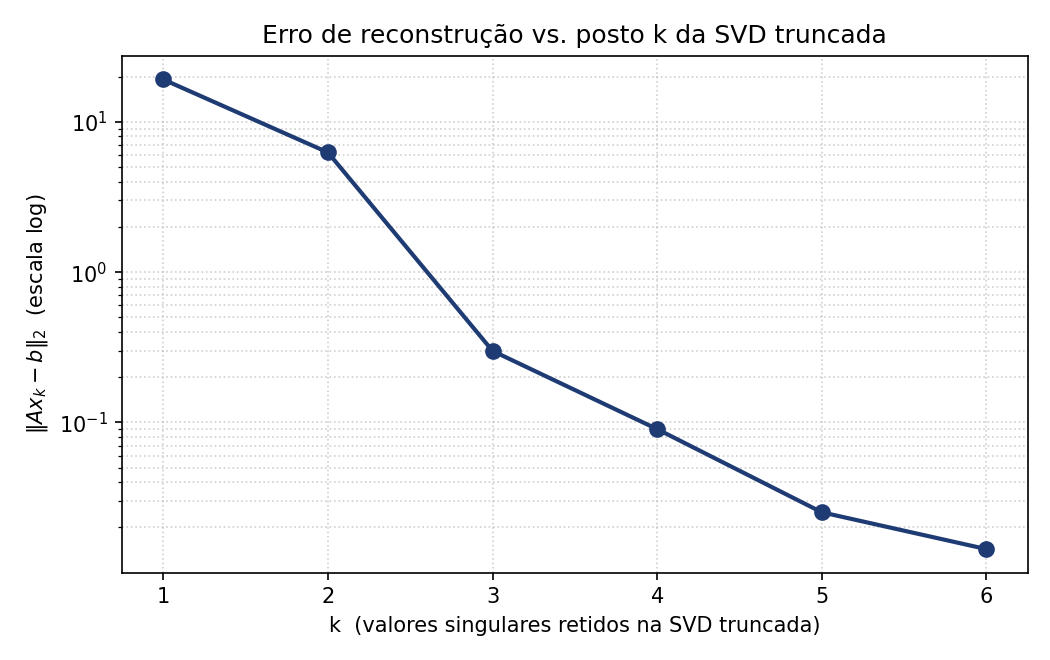
\includegraphics[width=0.78\textwidth]{fig_erro_rank.png}
\caption{Erro de reconstrução $\norm{Ax_k-b}_2$ em escala logarítmica versus o número $k$ de
valores singulares retidos. O erro cai rapidamente ao se incluírem os componentes dominantes.}
\label{fig:rank}
\end{figure}

O resultado ilustra um ponto importante neste experimento: os primeiros valores singulares carregam a maior parte da energia da matriz construída, enquanto os últimos, pequenos, pouco acrescentam à reconstrução e, quando há ruído nos dados, podem até atrapalhar. É esse o princípio da SVD truncada como técnica de \emph{regularização}; para aproximação matricial sem restrição adicional, o teorema de Eckart-Young garante que a SVD truncada produz a melhor aproximação de posto $k$ nas normas espectral e de Frobenius (ECKART; YOUNG, 1936; GOLUB; VAN LOAN, 2013; HANSEN, 2010).

\subsection{Análise do número de condição}

Por fim, examinou-se o impacto do condicionamento sobre a estabilidade numérica. Geraram-se
matrizes com $\kappa(A)$ variando de $1$ a $10^{10}$, perturbando-se o vetor $b$ com um erro
relativo fixo de $10^{-8}$ e medindo-se o erro relativo resultante na solução. A
Figura~\ref{fig:cond} mostra que o erro na solução tende a crescer com $\kappa(A)$,
acompanhando a escala prevista por $\kappa(A)\cdot\delta$: para $\kappa(A)=10^{8}$, um erro de
$10^{-8}$ na entrada já produz, neste ensaio, erro da ordem de $40\%$ na saída.

\begin{figure}[htbp]
\centering
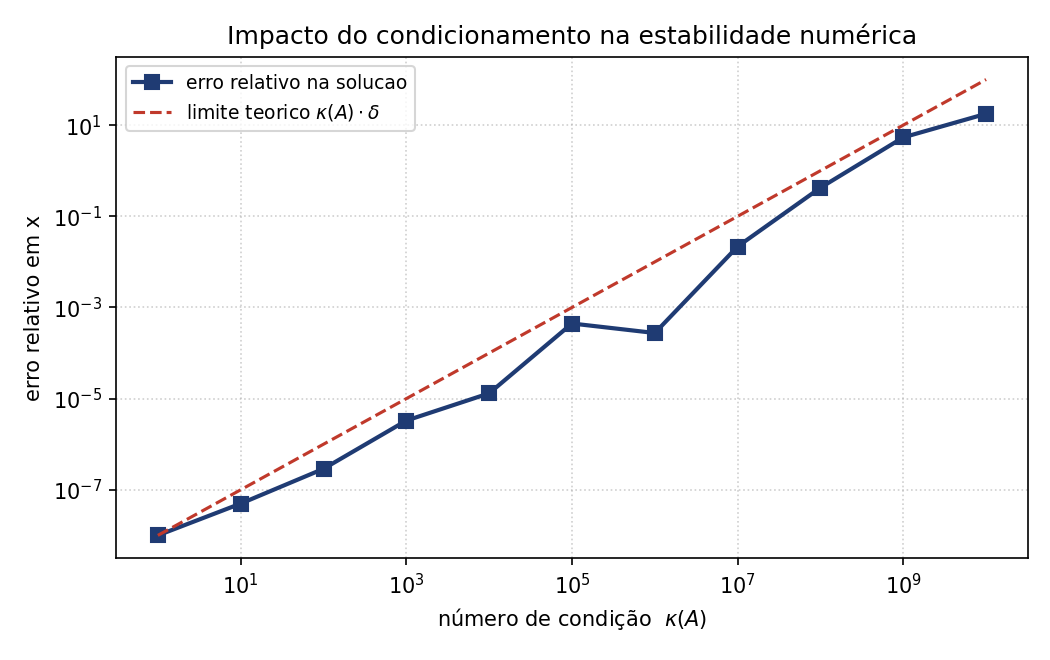
\includegraphics[width=0.78\textwidth]{fig_condicionamento.png}
\caption{Erro relativo na solução em função de $\kappa(A)$ (escala log-log). O erro acompanha
o limite teórico $\kappa(A)\cdot\delta$, o que mostra a perda de estabilidade em matrizes mal condicionadas.}
\label{fig:cond}
\end{figure}

Na prática, isso quer dizer que, quando $\kappa(A)$ é grande, nem o cálculo exato da pseudoinversa protege contra a amplificação dos erros já presentes nos dados. Em problemas inversos e dados ruidosos, a SVD truncada pode ajudar: ao descartar os valores singulares minúsculos, ela introduz viés, mas pode reduzir a variância e a sensibilidade ao ruído (HANSEN, 2010).

\section{Aplicações em Engenharia de Computação e Telecomunicações}

\subsection{Computação Gráfica: ajuste de curvas e compressão por SVD}

Em Computação Gráfica e processamento geométrico, a pseudoinversa aparece em vários problemas de ajuste de modelos a conjuntos de pontos. O ajuste polinomial por mínimos quadrados é o exemplo direto: dados pontos
$(x_i, y_i)$, monta-se a matriz de Vandermonde $V$ e resolve-se $V c = y$ por $c = V^{+} y$,
obtendo os coeficientes do polinômio que melhor aproxima os dados. A Figura~\ref{fig:ajuste}
mostra o ajuste de um polinômio de grau~5 a~18 pontos ruidosos, com erro quadrático médio de
$0{,}168$.

\begin{figure}[htbp]
\centering
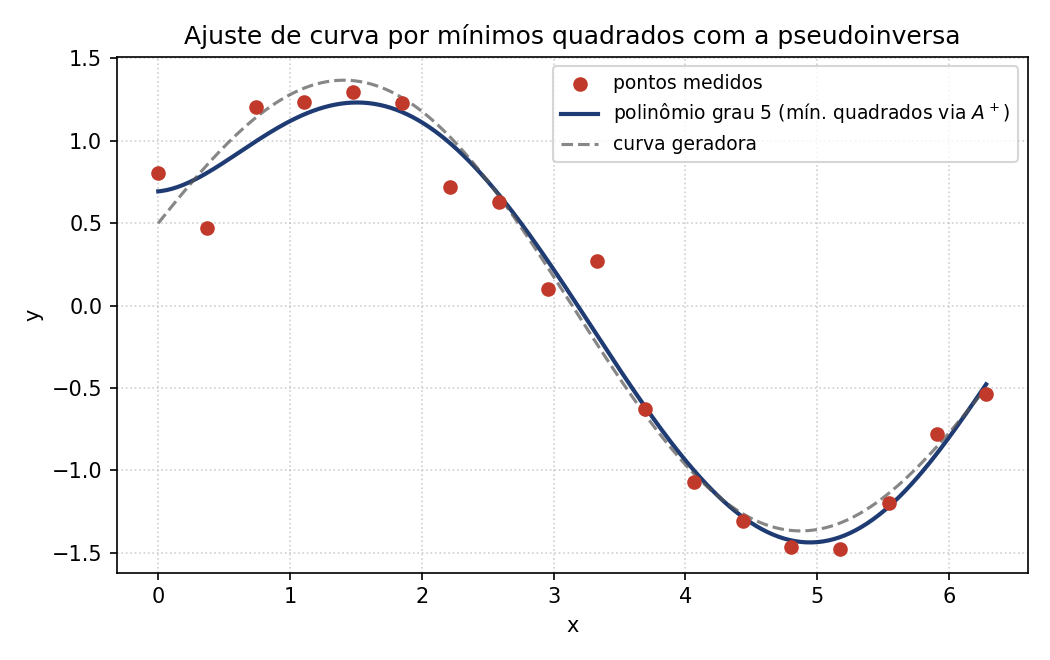
\includegraphics[width=0.80\textwidth]{fig_ajuste_curva.png}
\caption{Ajuste de curva por mínimos quadrados via pseudoinversa: pontos medidos, polinômio
ajustado ($c = V^{+}y$) e curva geradora.}
\label{fig:ajuste}
\end{figure}

O mesmo princípio vale para compressão e aproximação de imagens: uma imagem, vista como matriz, pode ser aproximada por sua SVD truncada de posto $k$, guardando só os componentes mais importantes no sentido de energia. Em visão computacional, problemas como calibração de câmeras e estimativa de transformações geométricas (\emph{homografias}) frequentemente levam a sistemas lineares resolvidos por mínimos quadrados ou SVD (HARTLEY; ZISSERMAN, 2004).

\subsection{Telecomunicações: estimação de canal MIMO}

Em sistemas MIMO (\emph{Multiple-Input Multiple-Output}), o sinal recebido modela-se como
$y = Hx + n$, onde $H$ é a matriz de canal. Um receptor de forçagem a zero (\emph{zero-forcing}) estima o sinal por
$\hat{x} = H^{+}y$ quando $H$ não é quadrada ou quando se formula o problema em mínimos quadrados. Esse procedimento cancela a interferência espacial no modelo linear ideal, mas pode amplificar ruído quando $H$ é mal condicionada; por isso o número de condição de $H$ é relevante para avaliar a confiabilidade da estimativa (TSE; VISWANATH, 2005).

\subsection{Aprendizado de máquina: regressão linear}

Na regressão linear por mínimos quadrados, a pseudoinversa fornece a solução de menor norma
$\theta = X^{+} y$, onde $X$ é a matriz de características; quando $X$ tem posto coluna completo, essa solução coincide com a obtida pelas equações normais. A regressão \emph{ridge}, por sua vez, não é simplesmente a pseudoinversa truncada: ela substitui o recíproco $1/\sigma_i$ por filtros amortecidos $\sigma_i/(\sigma_i^2+\lambda)$, reduzindo a influência de valores singulares pequenos (HASTIE; TIBSHIRANI; FRIEDMAN, 2009; HANSEN, 2010). Um conceito de 1920, portanto, continua presente em algoritmos estatísticos e de aprendizado de máquina.

% ===================== CAPITULO 3 - REFLEXAO ================================
\chapter{Reflexão: cálculo numérico, computação e engenharia}

O estudo da pseudoinversa deixa ver uma ideia mais geral: o cálculo numérico e a ciência da computação moderna estão profundamente ligados. A formulação algébrica de $\Ap$ existe desde 1920, mas seu uso prático em larga escala dependeu de algoritmos estáveis de SVD e de hardware capaz de executá-los. História e técnica andam juntas: muitos métodos nascem de necessidades computacionais e, depois de amadurecidos, ampliam o que a engenharia consegue fazer.

Para o engenheiro de computação e de telecomunicações, isso exige alguns conceitos que este trabalho ilustrou na prática. Um é a noção de \emph{erro} (absoluto, relativo, de arredondamento e de truncamento). Como lembra Aquino (2020), uma pequena perturbação pode ser amplificada até levar a uma resposta sem sentido, e o número de condição é o que mede esse risco. Outro é a \emph{estabilidade}: vimos que a forma via SVD da pseudoinversa é melhor que a equação normal por ser mais estável, embora as duas sejam ``corretas'' no papel. O terceiro é a \emph{escolha do método}: não adianta funcionar só na teoria; é preciso escolher a variante numericamente segura para o problema concreto.

Esse estudo também deixou clara a importância de validar resultados por mais de um caminho. Verificar os resíduos das quatro condições de Moore-Penrose e confrontar a implementação própria com uma rotina consagrada não é mero formalismo: é a aplicação prática do princípio, defendido por Aquino (2020), de que os erros devem ser minimizados ou, ao menos, identificados, empregando técnicas distintas para que os resultados sejam comparados. A regularização pela SVD truncada, por sua vez, ilustra um compromisso recorrente na engenharia: aceitar viés em troca de menor sensibilidade ao ruído.

Há, ainda, uma reflexão sobre o uso de bibliotecas prontas \emph{versus} a implementação
própria. Ferramentas como \texttt{pinv} do Scilab ou do NumPy resolvem o problema com uma única
linha, e é razoável usá-las na maior parte do tempo. Mas tratá-las como ``caixas pretas'' tem
riscos: a escolha do limiar de corte dos valores singulares, por exemplo, afeta silenciosamente
o resultado, e um usuário desavisado pode não perceber que sua matriz é mal condicionada.
Implementar a pseudoinversa do zero, como se fez aqui, revela essas decisões internas e forma o
julgamento necessário para usar as ferramentas prontas com responsabilidade.

Por fim, a computação continua influenciando os métodos numéricos. A computação de alto desempenho e as GPUs mudam o que é viável calcular em álgebra linear, otimização e simulação. Mesmo temas emergentes, como a computação quântica, podem alterar no futuro a forma de tratar certos problemas numéricos, mas ainda não substituem as técnicas clássicas no uso cotidiano. O cálculo numérico, portanto, não é um assunto encerrado; segue muito ativo.

% ========================== CONCLUSAO =======================================
\chapter*{Conclusão}
\addcontentsline{toc}{chapter}{Conclusão}

Este trabalho analisou a história do cálculo numérico e sua relação com a ciência da computação, com foco na pseudoinversa de Moore-Penrose. Voltando aos objetivos propostos, percorremos marcos da disciplina, de Arquimedes aos ambientes atuais como o Scilab e o Python, e vimos como os computadores digitais transformaram métodos antes impraticáveis em ferramentas de uso corrente.

No tema específico, mostrou-se que a pseudoinversa generaliza a inversa clássica para matrizes
quaisquer, sendo caracterizada de forma única pelas quatro condições de Moore-Penrose e
calculada de modo estável pela decomposição em valores singulares. A implementação
desenvolvida reproduziu $\Ap$ a partir da SVD com erro da ordem da precisão de máquina em
relação à rotina de referência, satisfez as quatro condições e resolveu corretamente os casos
sobredeterminado (mínimos quadrados) e subdeterminado (mínima norma). As análises de posto e de
condicionamento explicitaram o papel do limiar dos valores singulares como critério de
estabilidade (análogo ao critério de tolerância dos métodos iterativos) e o impacto do
número de condição sobre a propagação de erros.

As aplicações mostraram a importância do tema para a formação do engenheiro: ajuste de curvas e aproximação de imagens, estimação de canal em sistemas MIMO e regressão em aprendizado de máquina usam, direta ou indiretamente, ideias de mínimos quadrados, SVD e regularização. O aprendizado principal é simples: entender o que está por baixo da função de biblioteca, e não apenas chamá-la, é o que permite usá-la com segurança. Para frente, a computação de alto desempenho e as GPUs devem manter o cálculo numérico no centro dos problemas de álgebra linear de larga escala.

% ========================== REFERENCIAS =====================================
\chapter*{Referências}
\addcontentsline{toc}{chapter}{Referências}
\begingroup
\singlespacing
\setlength{\parindent}{0pt}
\setlength{\parskip}{0.9em}

AQUINO, F. J. A. de. \textbf{Tópicos de métodos numéricos com Scilab}: computação científica
para engenheiros. Rio de Janeiro: PoD Editora, 2020.

BABBAGE, C. \textbf{On the application of machinery to the computation of astronomical and
mathematical tables}. London: Royal Astronomical Society, 1822.

BEN-ISRAEL, A.; GREVILLE, T. N. E. \textbf{Generalized inverses}: theory and applications.
2. ed. New York: Springer, 2003.

BJERHAMMAR, A. Application of calculus of matrices to method of least squares; with special
references to geodetic calculations. \textbf{Transactions of the Royal Institute of Technology},
n. 49, 1951.

BOYER, C. B.; MERZBACH, U. C. \textbf{A history of mathematics}. 3. ed. Hoboken: Wiley, 2011.

BURDEN, R. L.; FAIRES, J. D. \textbf{Numerical Analysis}. 10. ed. Boston: Cengage Learning, 2015.

CERUZZI, P. E. \textbf{A history of modern computing}. 2. ed. Cambridge: MIT Press, 2003.

CHAPRA, S. C.; CANALE, R. P. \textbf{Métodos numéricos para engenharia}. 7. ed. Porto Alegre:
AMGH, 2016.

COOLEY, J. W.; TUKEY, J. W. An algorithm for the machine calculation of complex Fourier series.
\textbf{Mathematics of Computation}, v. 19, n. 90, p. 297--301, 1965.

ECKART, C.; YOUNG, G. The approximation of one matrix by another of lower rank.
\textbf{Psychometrika}, v. 1, n. 3, p. 211--218, 1936.

GOLUB, G. H.; KAHAN, W. Calculating the singular values and pseudo-inverse of a matrix.
\textbf{Journal of the Society for Industrial and Applied Mathematics, Series B: Numerical
Analysis}, v. 2, n. 2, p. 205--224, 1965.

GOLUB, G. H.; REINSCH, C. Singular value decomposition and least squares solutions.
\textbf{Numerische Mathematik}, v. 14, p. 403--420, 1970.

GOLUB, G. H.; VAN LOAN, C. F. \textbf{Matrix Computations}. 4. ed. Baltimore: Johns Hopkins
University Press, 2013.

HANSEN, P. C. \textbf{Discrete inverse problems}: insight and algorithms. Philadelphia: SIAM,
2010.

HARTLEY, R.; ZISSERMAN, A. \textbf{Multiple view geometry in computer vision}. 2. ed. Cambridge:
Cambridge University Press, 2004.

HASTIE, T.; TIBSHIRANI, R.; FRIEDMAN, J. \textbf{The elements of statistical learning}: data
mining, inference, and prediction. 2. ed. New York: Springer, 2009.

HIGHAM, N. J. \textbf{Accuracy and stability of numerical algorithms}. 2. ed. Philadelphia: SIAM,
2002.

METROPOLIS, N.; ULAM, S. The Monte Carlo method. \textbf{Journal of the American Statistical
Association}, v. 44, n. 247, p. 335--341, 1949.

MOLER, C. The origins of MATLAB. \textbf{MathWorks}, [s.d.]. Disponível em:
\url{https://www.mathworks.com/company/technical-articles/the-origins-of-matlab.html}.
Acesso em: 19 jun. 2026.

MOORE, E. H. On the reciprocal of the general algebraic matrix. \textbf{Bulletin of the
American Mathematical Society}, v. 26, p. 394--395, 1920.

NUMPY DEVELOPERS. \textbf{numpy.linalg.pinv} --- NumPy Manual. Disponível em:
\texttt{https://numpy.org/doc/stable/}. Acesso em: 19 jun. 2026.

PENROSE, R. A generalized inverse for matrices. \textbf{Mathematical Proceedings of the
Cambridge Philosophical Society}, v. 51, n. 3, p. 406--413, 1955.

STIGLER, S. M. \textbf{The history of statistics}: the measurement of uncertainty before 1900.
Cambridge: Harvard University Press, 1986.

STRANG, G. \textbf{Linear Algebra and Its Applications}. 4. ed. Belmont: Thomson Brooks/Cole,
2006.

TSE, D.; VISWANATH, P. \textbf{Fundamentals of wireless communication}. Cambridge: Cambridge
University Press, 2005.

TURING, A. M. On computable numbers, with an application to the Entscheidungsproblem.
\textbf{Proceedings of the London Mathematical Society}, s. 2, v. 42, n. 1, p. 230--265, 1937.

VON NEUMANN, J.; GOLDSTINE, H. H. Numerical inverting of matrices of high order. \textbf{Bulletin
of the American Mathematical Society}, v. 53, n. 11, p. 1021--1099, 1947.

WILKINSON, J. H. \textbf{Rounding errors in algebraic processes}. London: Her Majesty's Stationery
Office, 1963.

\endgroup

\end{document}